\documentclass[tikz,border=10pt]{standalone}
\usetikzlibrary{calc}
\begin{document}
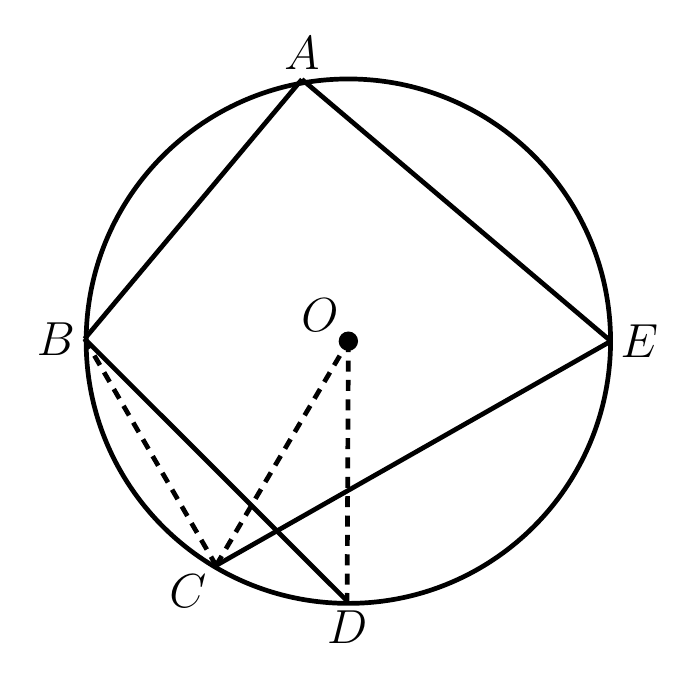
\begin{tikzpicture}[line join=round, font=\fontsize{17}{20.4}\selectfont]
\coordinate (A) at (-0.590,3.325);
\coordinate (B) at (-3.349,0.030);
\coordinate (C) at (-1.680,-2.849);
\coordinate (D) at (-0.016,-3.300);




\coordinate (O) at (0.000,0.000);
\coordinate (E) at (3.334,0.000);


\draw[line width=1.7pt] (O) circle (3.330);


\draw[line width=1.7pt] (A) -- (B);
\draw[line width=1.7pt] (A) -- (E);
\draw[line width=1.7pt] (B) -- (D);
\draw[line width=1.7pt] (E) -- (C);


\draw[line width=1.7pt, dash pattern=on 4pt off 3pt] (B) -- (C);
\draw[line width=1.7pt, dash pattern=on 4pt off 3pt] (C) -- (O);
\draw[line width=1.7pt, dash pattern=on 4pt off 3pt] (O) -- (D);


\fill (O) circle (3.500pt);


\node[above] at (A) {$A$};
\node[left] at (B) {$B$};
\node[right] at (E) {$E$};
\node[below left] at (C) {$C$};
\node[below] at (D) {$D$};
\node[above left] at (O) {$O$};
\end{tikzpicture}
\end{document}